\chapter{O preâmbulo}
No capítulo~\ref{sch:basic} vimos que o \emph{preâmbulo} é iniciado por
\begin{code}
  \documentclass[opcoes]{classe}
\end{code}

O \emph{preâmbulo}\index{preambulo@\emph{preâmbulo}} é completado com a inclusão
de pacotes que serão utilizados na \emph{informação}. O comando para inclusão de
um pacote\index{comando!usepackage@\lstinline+\usepackage+} segue a seguinte
sintaxe:
\begin{code}
  \usepackage[opcoes]{pacote}
\end{code}
onde \lcode{pacote} é o nome do pacote e \lcode{opcoes} é uma lista de
palavras chaves correspondente a opções do pacote. Nesse e nos próximos
capítulos será apresentado alguns dos pacotes existentes.

No \emph{preâmbulo} o usuário também pode definir seus
próprios comandos e ambientes\footnote{Não será abordado neste curso, uma ótima
fonte é \url{http://en.wikibooks.org/wiki/LaTeX/Customizing_LaTeX}}.

\section{Teclado e Idioma}
Na época que o TeX foi desenvolvido utilizava-se a codificação ASCII (American
Standard Code for Information Interchange) e, consequentemente, o LaTeX foi
desenvolvido para utilizar apenas os caracteres presentes na codificação ASCII.

As 52 letras (26 letras minúsculas + 26 letras maiúsculas) do alfabeto
americano, os dez dígitos indo-arábicos, seis sinais de pontuação
(\lstinline+, ; . ? ! :+) e quatro parenteses (\lstinline!( ) [ ]!). Todos estas
teclas são interpretadas como elas mesmas pelo LaTeX.

Na seção \ref{sss:basic:space} abordamos como o LaTeX interpreta o espaço e
enter (mudança de linha).

As teclas correspondentes a \lstinline!`!, acento grave, \lstinline!'!,
apóstrofe, e \lstinline!-!, hífen, são interpretadas pelo LaTeX de acordo com os
caracteres adjacentes.

Os seis símbolos matemáticos (\lstinline!* + = < > /!) são interpretados de
maneira diferentes quando no modo texto e no modo matemático\footnote{O modo
matemático é apresentado no capítulo \ref{sch:math}.}.

Existem, também, 13 símbolos especiais (\lstinline!# $ % & ~ _ ^ \ { } @ " |!)
que são interpretados pelo LaTeX de acordo com os caracteres adjacentes.

Os demais caracteres disponíveis no teclado, quando utilizados, costumam
produzir erro.

Para facilitar o uso do LaTeX em outros idiomas que não o inglês pode-se
utilizar alguma codificação diferente da ASCII para o arquivo \lcode{.tex}. Ao
utilizar uma codificação diferente da ASCII fazendo uso de caracteres não
presentes na ASCII é necessário utilizar o pacote \pkgname{inputenc} e informar
a codificação\footnote{A maioria das codificações são compatíveis com a ASCII e
por esse motivo se for utilizado apenas caracteres ASCII não é necessário a
inclusão do pacote \pkgname{inputenc}.} As codificações mais comuns são UFT-8 e
Latin1 sendo que para arquivos codificados com UFT-8 deve-se adicionar a
seguinte linha no preâmbulo
\begin{code}
  \usepackage[utf8]{inputenc}
\end{code}\index{pacote!inputenc@\pkgname{inputenc}}
enquanto que para arquivos codificados com Latin1
\begin{code}
  \usepackage[latin1]{inputenc}
\end{code}
Recomenda-se utilizar a codificação UFT-8 (Unicode) pois a Latin1 não possue
mais suporte desde 2004 (ver \url{http://pt.wikipedia.org/wiki/ISO_8859-1}) ou
apenas os caracteres definidos na codificação ASCII pois estes possuem a mesma
representação na maioria das codificações existentes.

É importante que o editor que esteja sendo usado também esteja configurado para
trabalhar com a codificação especificada. Quando uma codificação errada estiver
sendo usada, o editor pode trocar ou omitir alguns caracteres.

Ao gerar um arquivo \lcode{pdf} utilizando o LaTeX ocorre que copiar e colar um
fragmento de texto no \lcode{pdf} com caracteres que não esteja presentes na codificação
ASCII será preciso corrigir o fragmento. Para atenuar esse trabalho deve-se
utilizar o pacote \envname{fontenc}\index{pacote!fontenc@\envname{fontenc}}.

\section{Internacionalização}
Uma vez que parte considerável de uma obra produzida utilizando o LaTeX é feita
de maneira automática a internacionalização é importantíssima. No
desenvolvimento de software, internacionalização é o nome dado a capacidade de
um programa adequar-se aos padrões de diferentes países como, por exemplo, a
língua.

No LaTeX, a internacionalização é feita pelo pacote
\pkgname{babel}\index{pacote!babel@\pkgname{babel}} de Johannes L. Braams que
ajusta algumas macros de acordo com o idioma desejado, como a traduções de
alguns termos e uso de caixa alta. O pacote \pkgname{babel} possui as
seguintes opções para o idioma português: \lcode{portuges}, \lcode{portuguese},
\lcode{brazil}, \lcode{brazilian}. Maiores detalhes podem ser encontrados na
documentação do pacote\cite{Braams:2008:Babel}.

\section{Parágrafos}
Por padrão, o primeiro parágrafo de capítulo, seções, \dots, não é indentado.
Quando desejar-se indentar o primeiro parágrafo uma solução é utilizar o pacote
\pkgname{indentfirst}.

\section{Margens}
A configuração de margens\index{margens} no LaTeX pode ser feita nativamente,
utilizando o pacote \pkgname{geometry} ou o pacote \pkgname{fancyhdr}. A seguir
abordaremos o pacote \pkgname{geometry} e o estilo de página.

\subsection{\pkgname{geometry}}
O uso deste pacote é bastante simples, precisa-se apenas fazer a chamada do
pacote e atribuir valores para os parâmetros disponíveis. A seguir apresentamos
um exemplo:
\begin{code}
  \usepackage{geometry}
  \geometry{parametro = comprimento, ...}
\end{code}
ou
\begin{code}
  \usepackage[parametro = comprimento, ...]{geometry}
\end{code}\index{pacote!geometry@\pkgname{geometry}}

Podemos utilizar \lcode{comprimento} em qualquer unidade disponível no LaTeX, mm, cm
e outras. Já as opções para \lcode{parametro} mais utilizadas são apresentadas
na Tabela~\ref{tab:par_geometry} e ilustradas na Figura~\ref{fig:par_geometry}.
\begin{table}[h!tb]
  \centering
  \caption{Opções disponíveis para \lcode{parametro}, referente ao pacote \lcode{geometry}.}
  \label{tab:par_geometry}
  % File: geometry@latex-with-vim.tex
% This code is part of LaTeX with Vim.
% 
% Description: LaTeX with Vim is free book about Vim, LaTeX and Git.
% 
% Created: 30.03.12 12:19:38 AM
% Last Change: 30.03.12 12:19:44 AM
% 
% Author: Raniere Gaia Costa da Silva, r.gaia.cs@gmail.com
% Organization:  
% 
% Copyright (c) 2010, 2011, 2012, Raniere Gaia Costa da Silva. All rights 
% reserved.
% 
% This file is license under the terms of a Creative Commons Attribution 
% 3.0 Unported License, or (at your option) any later version. More details
% at <http://creativecommons.org/licenses/by/3.0/>.

\begin{tabular}{lp{0.8\textwidth}}
    \hline
    Código & Descrição \\ \hline
    \lcode{paperwidth} & Largura do papel. \\
    \lcode{paperheight} & Altura do papel. \\
    \lcode{textwidth} & Largura da caixa de texto. \\
    \lcode{textheigth} & Altura da caixa de texto. \\
    \lcode{top} & Margem superior. \\
    \lcode{bottom} & Margem inferior. \\
    \lcode{lefth} & Margem esquerda. \\
    \lcode{right} & Margem direita. \\ \hline
\end{tabular}

\end{table}
\begin{figure}[h!]
  \centering
  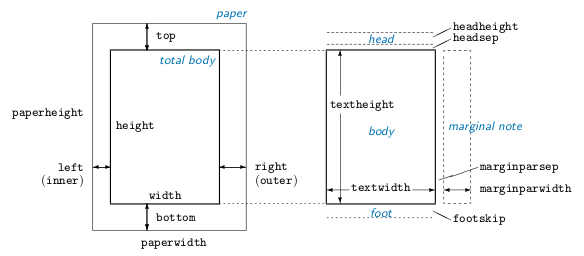
\includegraphics[width=0.8\textwidth]{figures/geometry_margin.png}
  \flushright Fonte: \cite{Umeki:2010:Geometry}
  \caption{Ilustração da opções disponíveis para \lcode{parametro} apresentadas na Tabela \ref{tab:par_geometry}.} \label{fig:par_geometry}
\end{figure}

\subsection{Estilo de página}
Existe um estilo de página definido como padrão\footnote{Corresponde ao estilo
\lcode{plain} apresentado na Tabela \ref{tab:par_style}.}, quando deseja-se
mudar o estilo em todo o documento pode-se utilizar o comando
\begin{code}
  \pagestyle{style}
\end{code}
e quando for necessário mudá-lo apenas na página atual utiliza-se o comando
\begin{code}
  \thispagestyle{style}
\end{code}

As opções para \lcode{style} são apresentadas na Tabela~\ref{tab:par_style}.
\begin{table}[htb]
  \centering
  \caption{Opções disponíveis para \lcode{style}.}
  \label{tab:par_style}
  % File: style@latex-with-vim.tex
% This code is part of LaTeX with Vim.
% 
% Description: LaTeX with Vim is free book about Vim, LaTeX and Git.
% 
% Created: 30.03.12 12:19:38 AM
% Last Change: 30.03.12 12:19:44 AM
% 
% Author: Raniere Gaia Costa da Silva, r.gaia.cs@gmail.com
% Organization:  
% 
% Copyright (c) 2010, 2011, 2012, Raniere Gaia Costa da Silva. All rights 
% reserved.
% 
% This file is license under the terms of a Creative Commons Attribution 
% 3.0 Unported License, or (at your option) any later version. More details
% at <http://creativecommons.org/licenses/by/3.0/>.

\begin{tabular}{lp{0.8\textwidth}}
    \hline
    Código & Descrição \\ \hline
    \lcode{plain} & Imprime os números de página no centro do pé da página. \\
    \lcode{headings} & No cabeçalho de cada página imprime o capítulo que está sendo processado e o número da página. O pé da página fica vazio. \\
    \lcode{empty} & Coloca tanto o cabeçalho como o pé da página vazios.
\end{tabular}

\end{table}

Aos interessados em criar um estilo próprio, sugere-se utilizar o pacote
\lcode{fancyhdr}.
